\documentclass[11pt, article, colorback]{article}
\usepackage{geometry}                % See geometry.pdf to learn the layout options. There are lots.
\geometry{letterpaper}                   % ... or a4paper or a5paper or ... 
%\geometry{landscape}                % Activate for for rotated page geometry
%\usepackage[parfill]{parskip}    % Activate to begin paragraphs with an empty line rather than an indent
\usepackage{graphicx}
%\usepackage{amssymb}
\usepackage{epstopdf}
\usepackage{subfigure}
\usepackage{verbatim}
\usepackage{hyperref}
\usepackage{array}
\usepackage{url} 
\usepackage{listings}
\lstset{language=C,
basicstyle=\footnotesize,
frame=single,
tabsize=2}
\renewcommand{\UrlBreaks}{\do\/\do\a\do\b\do\c\do\d\do\e\do\f\do\g\do\h\do\i\do\j\do\k\do\l\do\m\do\n\do\o\do\p\do\q\do\r\do\s\do\t\do\u\do\v\do\w\do\x\do\y\do\z\do\A\do\B\do\C\do\D\do\E\do\F\do\G\do\H\do\I\do\J\do\K\do\L\do\M\do\N\do\O\do\P\do\Q\do\R\do\S\do\T\do\U\do\V\do\W\do\X\do\Y\do\Z}
\usepackage{amsmath, amsthm}

\DeclareGraphicsRule{.tif}{png}{.png}{`convert #1 `dirname #1`/`basename #1 .tif`.png}

\title{{CompLACS Robot Arm Evaluation Scenarios}}
%\institution{Institut fuer Intelligente Autonome Systeme}

\author{Christian Daniel \\ Gerhard Neumann \\ Jan Peters \newline }
%\date{}                                           % Activate to display a given date or no date

\begin{document}
\maketitle

\begin{abstract}This document contains a description of the robot-arm evaluation scenarios developed by the IAS at TU-Darmstadt for the CompLACS project. 
The goal of the software described in this document is to have a common platform that allows for easy implementation, evaluation and 
comparison of different robot evaluation platforms, experiments and learning algorithms. 
We use 8 different scenarios which are the Pole-Balancing, the Ball-on-a-Beam, the Ball-in-a-Cup, the  Ball-Padding,
Ball-Bouncing, Beer-Bong, Tetherball and the Casting task. All tasks are simulated using the SL simulation toolbox. We will first start with an introduction to SL and subsequently present the 8 individual tasks. Each task will be described in terms of the objective, the setup and its difficulties.  An installation guide of SL and a short tutorial of 
how to program controllers for the tasks can be found in the appendix.
\end{abstract}

\newpage \tableofcontents \newpage

\section{The SL Tools \& Environment}
%%%%%%%%%%%%%%%%%%%%%%%%%%%%%%%%%%%%%%%
%The scenarios are simulated using the
%SL tools [CITE] developed by the Computational Learning and Motor Control at University of Southern California\footnote{Jan Peters is part of %this group since starting his PhD in 2001}. 
%SL is already used by various other institutions (e.g. the Max Planck institute in Tuebingen, CMU in the USA, ATR 
%in Japan, etc.), allowing for easy cooperation and joint projects between those labs. It is constantly 
%being improved and kept up to date.

SL \cite{Schaal:2006tq} provides a rigid body simulation environment that enables researchers to easily implement and evaluate experiments on multiple robotic 
platforms with accurate physical models and high speed physics, making it suitable for a wide range of tasks from high 
precision grasping and manipulation tasks to high speed hitting or throwing tasks such as table tennis or dart throwing.  
It is implemented using the C programming language and has additional capabilities 
for evaluating results in Matlab. 

SL can be used in two different modes: simulation and real time control. In simulation mode, we can test new tasks and 
methods with an accurate physical simulation of the robots before testing it on the real 
system. This facilitates the setup of potentially dangerous (to the robot or its environment) or time 
consuming experiments. In the real-time control mode, the same controllers can be used to 
control the real robot, which makes the development and testing of new algorithms feasible in 
short time frames. The SL tools already contain a rigid-body physics simulation, which allows realistic simulation of highly dynamic movements
with robot manipulators. This allows for simple implementations of the controllers for the given tasks as it already contains basic robot control strategies such as
inverse dynamics control, control with gravity compensation or task-space control in the end-effector space. Controllers for the different tasks are implemented in C as they
also need to fulfill real-time requirements when controlling the real robot instead of the simulation. 

In general, robots may be controlled in two different manners. One is joint space control and the other is task space control. 
In joint space control we directly control the robots joint angles by setting the desired joint acceleration or the joint angles. It is often used in scenarios where highly-dynamic movements 
are required to fulfill a certain task. For task space control we directly want to control to the position of the robots end-effector in task 
space coordinates, thus the joint angle configuration of the robot is abstracted. It is frequently used for experiments where precision is important, e.g. grasping tasks. 
SL facilitates the use of either one control method by providing functions that perform all the necessary computations. For 
joint space control the user only has to pass the desired joint angles and velocities to the inverse dynamics which will then compute 
all necessary forces and apply them to the robot actuators. For task space control, the user only has to pass the desired 
end-effector coordinates to the inverse kinematics function which will return the required joint angles and velocities. These can then 
again be passed to the inverse dynamics to compute and apply the forces. 

For a more detailed description of how to implement controllers in SL, we refer to the 
appendix of this document, which also contains an installation guide of SL. 

\begin{figure}
{\centering
\mbox{\subfigure[WAM joints]{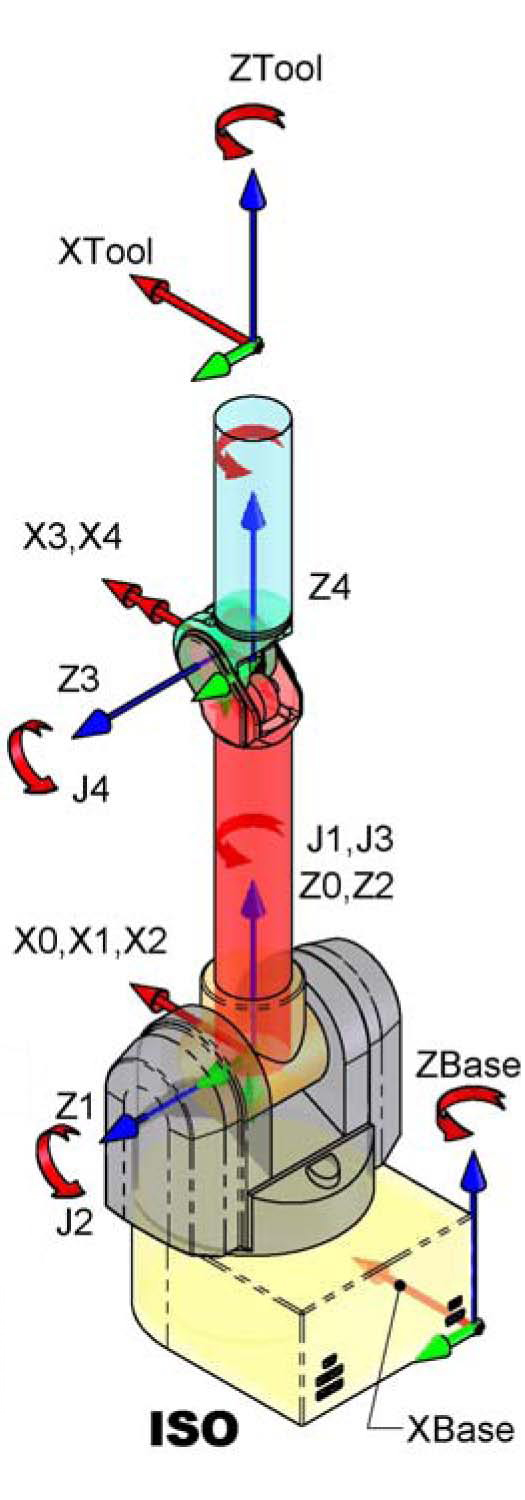
\includegraphics[width=1.7in]{Pics/WAM.jpg}}\quad
\subfigure[Simulated WAM]{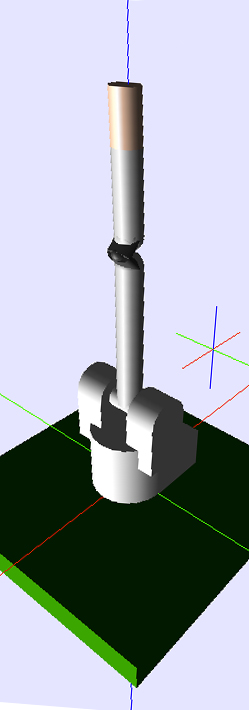
\includegraphics[width=1.7in]{Pics/WAMSim.jpg} }}
\caption{A drawing of the Barrett WAM showing its joints and a screen-shot of the simulated version} \label{pic:WAM}}
\label{pic:wam}
\end{figure}

For all tasks described in this document, we are using the Barrett Whole Arm Manipulator 
(WAM). Note, however, that SL already includes a variety of other robots such as the BioRob or the
Mitsubishi PA-10 arm and extending the simulator to include additional platforms is straightforward.

The Barrett WAM, as depicted in Fig. \ref{pic:wam}, is a seven degrees of freedom (DoF) robotic arm that is used for all of the experiments 
presented in this document. The WAM is a commonly used robotic platform. Its length is about one meter and it can support
a payload of up to three kilograms. It is available in different models, from three to seven DoF and with different maximum actuation 
forces. In the following we assume the WAM model to have the full 7 DoF and high speed actuation capabilities, as it is 
required for some of the more dynamic experiments. The WAM usually has some sort of end-effector attached. This end-effector could be either 
one of the WAM specific end-effector types like the Barrett Hand or the Barrett haptic ball, but it may also be any custom made kind 
of end-effector like the table tennis racket that is used in many of the presented experiments. 




\newpage
\section{Robot-Arm Evaluation Tasks}
%
All the task are usually learned in an episodic setup, i.e. we start from a single (or small set of different) initial states, execute our policy for a (usually fixed) amount
of time and gather the reward for the episode. Subsequently we again reset the simulation (drive the robot to its initial position and reset environment properties) and collect data for a new episode.
 After performing several episodes we usually update our policy. 

We now give a quick overview on the general work flow of a task on the example of the 
tetherball task. The most important function for each task is the {\em run\_*\_task function}, in our case it is {\em run\_tetherball\_task} 
which is called once during every simulation or control cycle. This function should be used with following skeleton :
%\newpage
\begin{lstlisting}
static int run_tetherball_task(void) 
{
	//Declare your variables here, then initialize them	
	if(firsttime) 
	{
		// initialize my static variables 
	}    

	//Simulate the physics of the environment
	sim_tetherball_state(FALSE);	
	if (goInit)
	{
		init_tetherball_task();
	}   
	
	if (playback)
	{
		double rewardTimeStep = getRewardStep();
		// Control my robot by setting joint_des_state
		// Put your code here...
	}	
	if (finishedEpisode)
	{		
		double rewardEpisode = getRewardEpisode();
		// Update my policy...
		// Put your code here...
	}  
	// Checks whether the trajectory might damage the robot
	check_range(joint_des_state);   
	// Computes Inverse Dynamics Control Law
	SL_InvDyn(joint_state,joint_des_state,endeff, &base_state, &base_orient);     
	
	return TRUE;
}
\end{lstlisting}
\lstset{frame=none}
Each environment is provided with the {\em sim\_*\_function} which simulates additional objects connected to the task (such as a ball) and also sets important variables needed for the work flow (e.g. {\em goInit, playback, finishedEpisode})
and also updates the current reward values. This function should be called before performing any control action. If the flag playback is set, the user has to control the robot. The reward for the last time step can be accessed with the function
{\em get\_*\_rewardstep}. If the {\em finishedEpisode} flag has been set, the episode is terminated and the user can access the reward collected throughout this episode by calling {\em get\_*\_rewardepisode}. Each environment is also 
provided with an init function {\em init\_*\_task} which resets the simulation and drives the robot to (one of) the given initial positions. 
%
%
\subsection{Ball-on-a-Beam}
%%%%%%%%%%%%%%%%%%%%%%%%%%%%%%%%%%%%%%%
\begin{figure}
\centering
 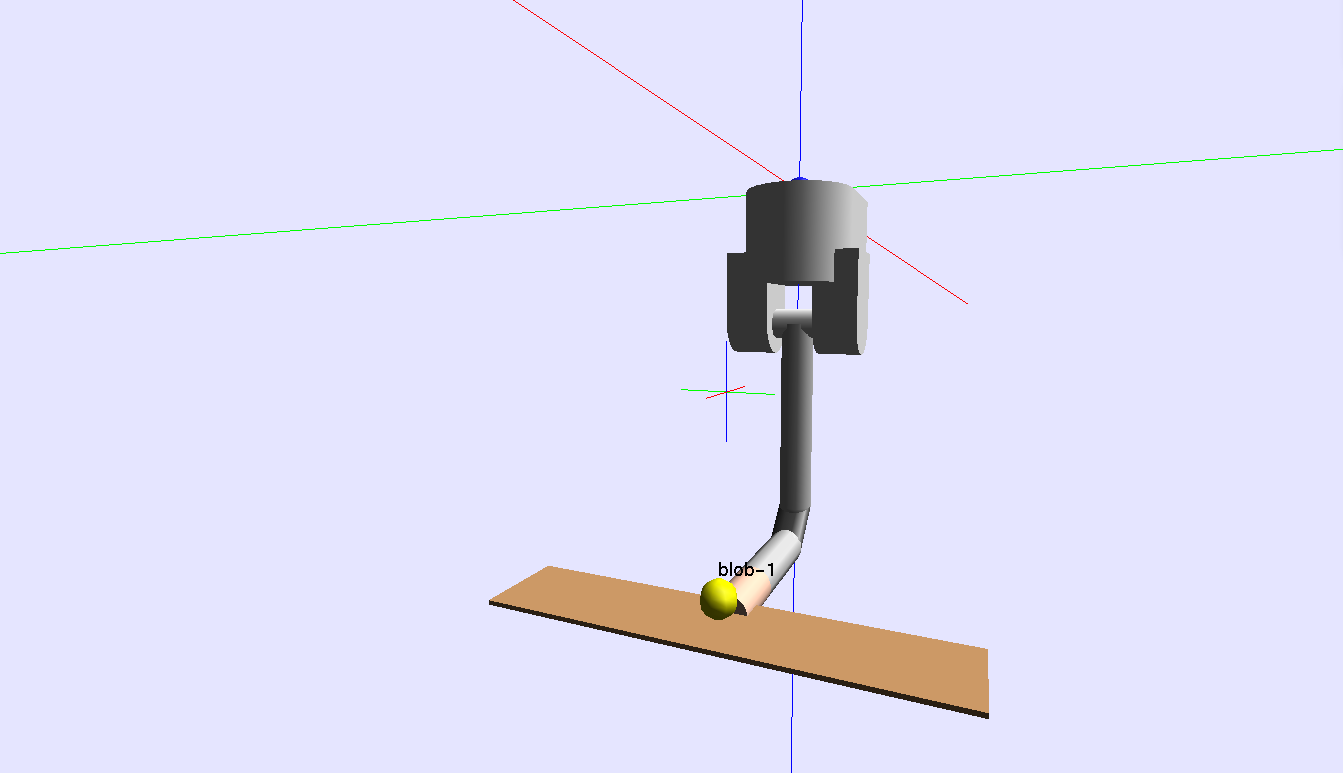
\includegraphics[width=0.8\textwidth]{Pics/BallOnBeam.png}
  \caption{A picture of the ball on a beam task simulation.}
  \label{pic:poleBalancing}
\end{figure}
%
\textbf{Objective:} Balance a ball on a beam while minimizing energy consumption. \\ \\
%
\textbf{Setup:} We are using the WAM with a beam attached to the end-effector.
		We initialize the beam in a horizontal pose and place a ball on top of it. The ball 
		is restricted to move in one dimension only (sideways).
		 \\ \\
%
\textbf{Description:}
The ball on a beam task is the easiest of the tasks presented in this document. A beam is attached 
to the robot, such that the robot can control the beams rotation directly by rotating its last joint. 
For the experiment, a ball is placed on the beam and the robot now has to hold the beam, such 
that the ball stays balanced at the centre of the beam. While the ball can fall off at either end of the beam, 
it cannot fall off to the sides of the beam. To ensure that this does not happen, the beam is framed  
along its long-sides. Constraining the balls motion in this way makes the task relatively easy to learn and thus 
appropriate as an introduction to the SL toolbox and the WAM.
		\\  \\
%
\textbf{Code Dependencies:} The following task specific variables and function calls should be helpful to 
successfully complete the pole balancing task. These are: \\
\begin{tabular}{ m{7cm} m{4cm}}
\begin{lstlisting}
Max reward up to this time step
Final reward
Simulate the physics
\end{lstlisting}
& \begin{lstlisting}
static int getRewardStep(void);
static double getRewardEpisode(void);
int sim_ballOnBeam_physics(int);
\end{lstlisting}
\end{tabular} \\





\subsection{Pole-Balancing} \label{sec:poleBalancing}
%%%%%%%%%%%%%%%%%%%%%%%%%%%%%%%%%%%%%%%
\begin{figure}
\centering
 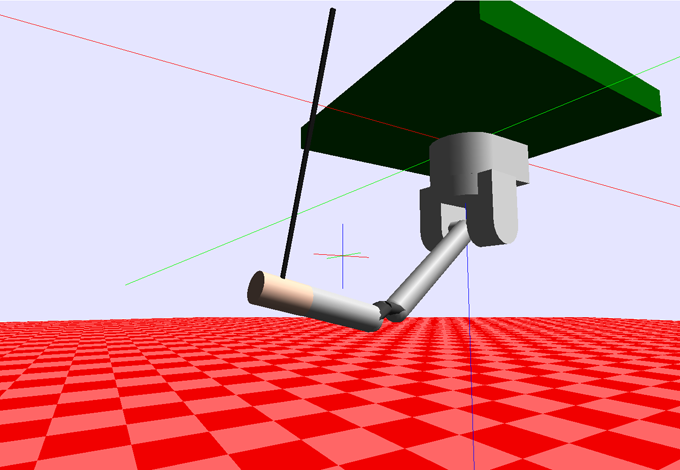
\includegraphics[width=0.8\textwidth]{Pics/PoleBalancing.png}
  \caption{A picture of the pole balancing simulation.}
  \label{pic:poleBalancing}
\end{figure}
%
\textbf{Objective:}	 Balance a pole such that it stays upright while minimizing energy consumption \\ \\
%
\textbf{Setup:}	We are using the WAM with a pole attached to the end-effector. 
We leave the last joint (rotary joint at the end-effector) non actuated. The pole 
has to be swung up from an initial position and be balanced upright.  \\ \\
%
\textbf{Description:}
Pole balancing, as shown in Fig.  \ref{pic:poleBalancing}, is a task that is inspired by both human artistic presentations 
as well as the 
widely used cart pole task. In the classical cart pole task, a cart is fixed on a rail with limited size by an articulated prismatic
joint. A pole is subsequently fixed to the front of the cart by a non articulated revolutionary joint. The cart can be accelerated 
along the axis of the rail as long as it does not reach the limits of the rail. The objective in that task is to first swing 
up the pole such that it is standing upright and then to balance the pole such that it keeps its upright position. 

In the presented pole balancing task, the setup differs in that we do not limit our selves to a single DoF. Instead we 
have to control all of the WAMs DoF, less the last one which we leave unarticulated. This adaptation of course makes the task 
harder to achieve. 
The objective of the task remains the same as in the cart pole task, the pole has to be first swung up and subsequently 
balanced upright. 

The difficulty of this task mainly depends on the length of the pole. The length of the pole determines how easily the 
pose of the pole is disturbed, i.e., how fast the robot has to react to stabilize the pole. A shorter pole is harder to keep 
upright than a longer pole. Additionally, it may be interesting to see how stable a given approach is to malfunction of 
one or more of the joints. To simulate this, one could learn a policy that successfully stabilizes the pole and then switch 
off the articulation of one of the joints.
This task is particularly interesting as a benchmark task since most available learning algorithms have at some point 
been tested on either a cart pole or a pole balancing task, making a meaningful comparison of approaches easier.		\\  \\
%
\textbf{Code Dependencies:} The following task specific variables and function calls should be helpful to 
successfully complete the pole balancing task. These are: \\
\begin{tabular}{ m{7cm} m{4cm}}
\begin{lstlisting}
pole orientation
pole angular speed
Final reward
Simulate the physics
\end{lstlisting}
& \begin{lstlisting}
q
dq
static double getRewardEpisode(void);
int sim_polebalancing_state(int);
\end{lstlisting}
\end{tabular} \\

		



\subsection{Ball-in-a-cup}
%%%%%%%%%%%%%%%%%%%%%%%%%%%%%%%%%%%%%%%
\begin{figure}
\centering
 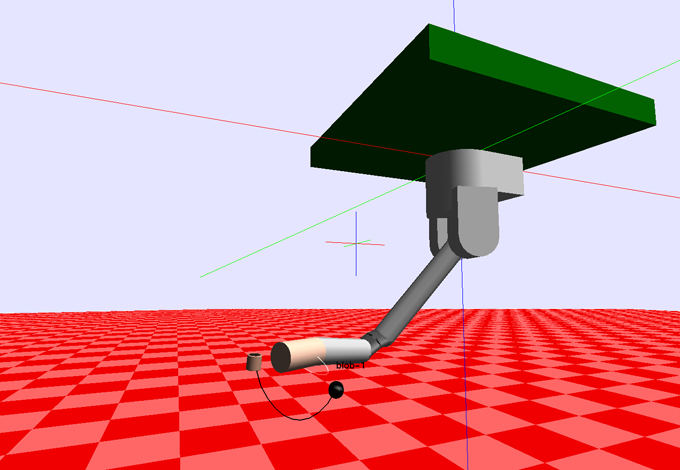
\includegraphics[width=0.8\textwidth]{Pics/BallInACup.png}
  \caption{A picture of the ball in a cup simulation.}
  \label{pic:biac}
\end{figure}
%
\textbf{Objective:} Swing up a ball that is fixed to a string and catch it with a cup. \\ \\
%
\textbf{Setup:}  We are using a cup as end-effector. To the bottom of the cup we attach an elastic string 
that holds a ball. We model the physics of the ball in free flight as well as the constrained motion under
an extended string.  \\ \\
%
\textbf{Description:}
This task, as shown in Fig. \ref{pic:biac}, is inspired by a children's game, where an elastic string is fixed to the bottom of a cup and a 
ball is fixed to the other end of the string. In order to allow the robot to learn the task, we fix the cup with the 
string (the ball is attached to this string) at the end-effector of the robot.
The objective of this task is to use the dynamics of ball to 
finally catch the ball with the cup. This task could theoretically be broken down into two subtasks. One being the 
swinging up of the ball and the second being the catching of the ball after it has been swung up and is on 
its way down. However, the robot does not have any prior information on the modularity of task and has to 
infer the two stages of the task from experience. 

The task is initialized in the same position for each each trial, that is with the the ball hanging down from the cup 
in a stable position without any velocities. For this task, it is not necessary to introduce any noise into 
the initialization since we start in a stable position and the robot will destabilize the system in order to achieve the objective. 

The difficulty of this task depends on various variables such as the diameter of the cup, the diameter of the ball, 
the mass of the ball, the length of the string and the elasticity of the string. A bigger ball or a more elastic string 
make this task harder, while a larger cup makes the task easier to learn. The effect of the length of the string is 
not as easy to predict. While in general a shorter string makes the system faster and thus more difficult, a very short string 
that only allows the ball to enter the cup could make the task easier again. 
		\\  \\
%
\textbf{Code Dependencies:} The following task specific variables and function calls should be helpful to 
successfully complete the pole balancing task. These are: \\
\begin{tabular}{ m{7cm} m{4cm}}
\begin{lstlisting}
Cup position
Cup speed 
Cup orientation
Ball position
Final reward
Simulate the physics
\end{lstlisting}
& \begin{lstlisting}
cup_state.x
cup_state.xd
cup_orient.q
blobs[1].blob.x
static double getRewardEpisode(void);
int sim_biac_state(int);
\end{lstlisting}
\end{tabular} \\


\subsection{Ball-Paddling}
%%%%%%%%%%%%%%%%%%%%%%%%%%%%%%%%%%%%%%%
\begin{figure}
\centering
 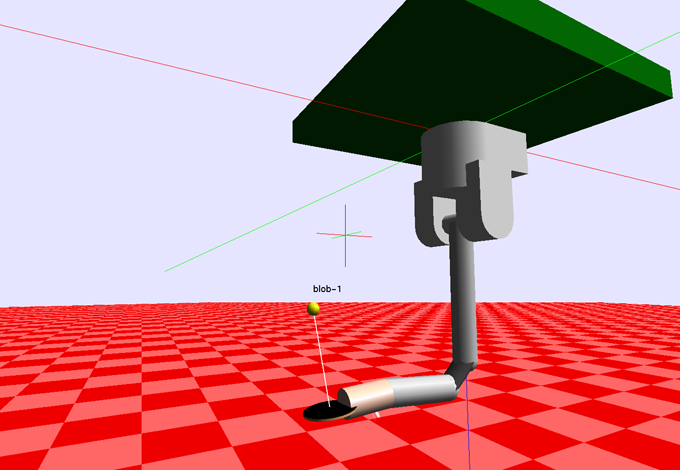
\includegraphics[width=0.8\textwidth]{Pics/PaddleBall.png}
  \caption{A picture of the ball paddling simulation.}
  \label{pic:ballPaddling}
\end{figure}
%
\textbf{Objective:}  Repeatedly pad a ball that is attached to a string with a racket without getting unstable. \\ \\
%
\textbf{Setup:}  We use the WAM with a racket as end-effector. To the middle of the racket we attach an 
elastic string that holds a ball. We model the physics of the ball in free flight as well as the constrained motion 
with an extended string.  \\ \\ 
%
\textbf{Description:}
In this task, as shown in Fig. \ref{pic:ballPaddling}, the objective is to find a stable, rhythmic motion that enables the robot to repeatedly hit a ball 
with a paddle. The setup of the task is such, that the ball is fixed to a highly elastic string and the string itself 
is fixed to the center of the racket. The racket is mounted directly 
as end-effector to the robot. When the robot hits the ball with the racket, the string extends and eventually draws the ball back to the 
racket. 

This task is quite difficult to learn for humans, especially if they do not have a well trained sense of fast rhythmic motions, 
e.g., by playing the drums. Every deviation from either the correct frequency or hitting angle introduces an error into the 
next contact with the ball. 

In general, the difficulty level of this task is mainly governed by the length of the string and the size of the racket. Other factors 
like the mass and size of the ball or the elasticity of the string may also be taken into account. This task is easiest to learn with 
a string length that is neither too short nor too long. Very short string lengths require very fast motions, where large string lengths 
introduce more errors. 
		\\  \\
%
\textbf{Code Dependencies:} The following task specific variables and function calls should be helpful to 
successfully complete the pole balancing task. These are: \\
\begin{tabular}{ m{7cm} m{4cm}}
\begin{lstlisting}
Ball position
Ball speed
Final reward
Simulate the physics
\end{lstlisting}
& \begin{lstlisting}
ball_state.x
ball_state.xd
static double getRewardEpisode(void);
int sim_paddleball_state(int);
\end{lstlisting}
\end{tabular} \\



\subsection{Ball-Bouncing}
%%%%%%%%%%%%%%%%%%%%%%%%%%%%%%%%%%%%%%%
\begin{figure}
\centering
 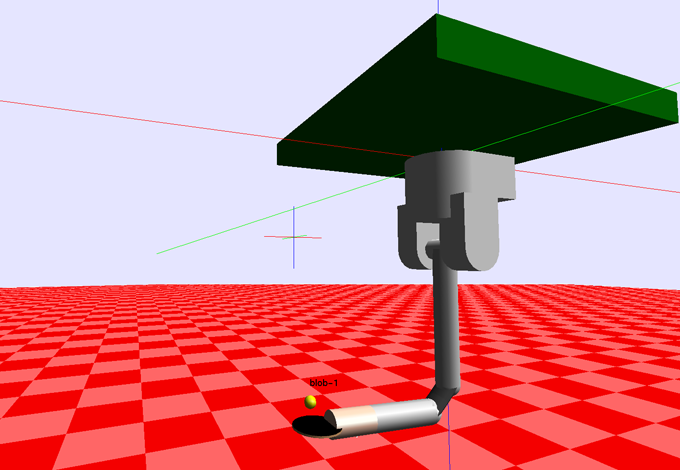
\includegraphics[width=0.8\textwidth]{Pics/Bouncing.png}
  \caption{A picture of the ball bouncing simulation.}
  \label{pic:ballBouncing}
\end{figure}
%
\textbf{Objective:} Repeatedly bounce a free floating ball with a tennis racket, without the ball hitting the floor. \\ \\
%
\textbf{Setup:}  We use the WAM with a tennis racket as end-effector. Initially the ball is lying on the racket. The 
ball is not fixed to the racket or robot in any way. \\ \\
%
\textbf{Description:}
The objective of this task, as shown in Fig. \ref{pic:ballBouncing}, is to continuously bounce a ball with a racket. 
This is a popular task amongst children and students of racket sports as it trains the understanding of the 
systems dynamics as well as the handling of the racket itself. As such it is also useful for robotics not only 
as stand alone benchmark task but also as part of a more complex task such as playing tennis. 

In this task, the racket is fixed to the robot as end-effector and the ball is not attached to the environment or the robot. 
In the initial state, the racket is oriented such that its surface is parallel to the ground and the ball is placed 
on the racket. The robot has to learn how to first get the ball to bounce off the racket and then how 
to continuously keep the ball bouncing in a stable rhythmic motion. However, the robot is not made aware 
of the two stages involved in this task and has to extract this information by learning. 

The difficulty of this task is mainly influenced by the racket size and the `elasticity' of the racket. The elasticity 
of the racket corresponds inversely to the tightness of the strings on a real tennis racket. To make the task harder, the 
elasticity of the racket can be increased. 
		\\  \\
%
\textbf{Code Dependencies:} The following task specific variables and function calls should be helpful to 
successfully complete the pole balancing task. These are: \\
\begin{tabular}{ m{7cm} m{4cm}}
\begin{lstlisting}
Ball position
Ball speed
Final reward
Simulate the physics
\end{lstlisting}
& \begin{lstlisting}
ball_state.x
ball_state.xd
static double getRewardEpisode(void);
int sim_bounceball_state(int);
\end{lstlisting}
\end{tabular} \\


\subsection{Beer Pong}
%%%%%%%%%%%%%%%%%%%%%%%%%%%%%%%%%%%%%%%
\begin{figure}
\centering
 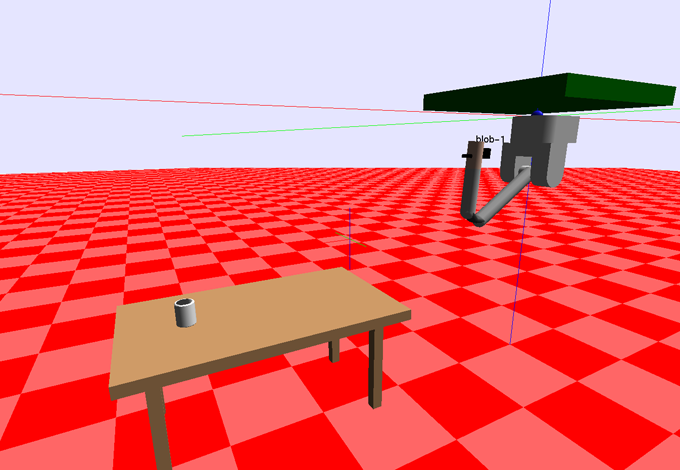
\includegraphics[width=0.8\textwidth]{Pics/BeerPong.png}
  \caption{A picture of the beer pong simulation.}
  \label{pic:beerPong}
\end{figure}
%
\textbf{Objective:} The robot is supposed to throw a ball on a table such that it bounces off the surface
and subsequently lands in a cup. \\ \\
%
\textbf{Setup:}  We use the WAM and fix the ball to its end-effector. In front of the WAM we place a table 
with a cup on it. Upon initialization the ball is fixed to the WAM and gets released during the throwing motion. \\ \\
%
\textbf{Description:}
This task more complicated to set up, as shown in Fig. \ref{pic:beerPong}. In this task the objective is to throw a ball such that it bounces off a surface 
into a cup placed on the same surface. The complexity of this task stems from the difficulty of actually throwing 
a ball with a robot, which involves accurate control of the robot's hand and its fingers, which is a complex task 
of its own. Given that we want to solve the dynamic throwing task and are in this setup less interested in the control 
of the robot hand, we replace the hand in simulation by a stick and a release mechanism. The ball is fixed to the end-effector 
of the robot until the controller relays a release signal, at which time the ball will be released from the end-effector 
and transition into free flight mode. 

Once the ball is in free flight mode, the robot does not have any control over its path, thus the policy to be learned 
has to find the right release velocities and release position. 

Apart from the discussed difficulties of actually releasing a ball in a throwing motion, the main challenges in this task 
are represented by the ball size as well as the cup diameter and height. In addition, the parameters describing the 
surface position, height, extension and elasticity may be of interest. To further increase the difficulty of this task, one 
might conceive scenarios where the surface is broken, such that the ball has only very limited areas where contact 
with the surface is possible before landing in the cup. One could also implement a slanted surface or a setup requiring 
multiple bounces of the ball to complete the objective. 
		\\  \\
%
\textbf{Code Dependencies:} The following task specific variables and function calls should be helpful to 
successfully complete the pole balancing task. These are: \\
\begin{tabular}{ m{7cm} m{4cm}}
\begin{lstlisting}
Cup position
Table position
Table height
Table length
Table width
Final reward
Simulate the physics
\end{lstlisting}
& \begin{lstlisting}
cup_state
table_height
table_length
table_width
static double getRewardEpisode(void);
int sim_beerpong_state(int);
\end{lstlisting}
\end{tabular} \\


\subsection{Tetherball-Target-Hitting}
%
\begin{figure}
{\centering
\mbox{\subfigure[Children's tetherball]{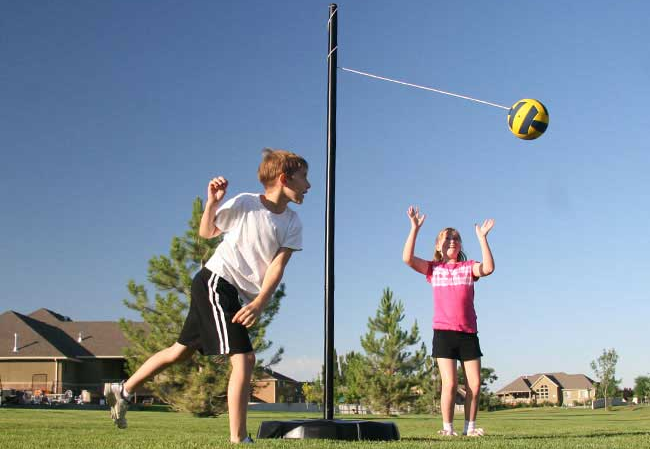
\includegraphics[width=3in]{Pics/Tetherball.png}}\quad
\subfigure[Robot tetherball]{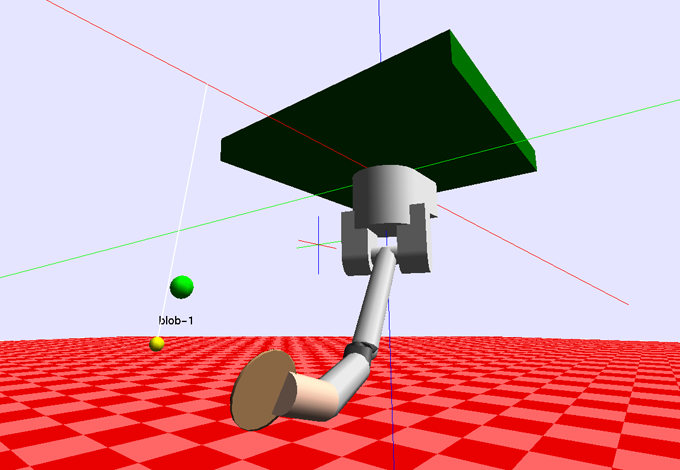
\includegraphics[width=3in]{Pics/TetherballSim.png} \label{pic:tetherball} } }
\caption{The original and adapted version of tetherball. (a) shows the original form of tetherball as children's game, 
where two children play against each other and (b) shows the robot tetherball setup, where the pole has been replaced
and the robot instead has to hit a target with the ball.} }
\end{figure}
%%%%%%%%%%%%%%%%%%%%%%%%%%%%%%%%%%%%%%%
%
\textbf{Objective:} Hit a ball that is hanging from the ceiling with a racket such that the ball comes as close as possible to a given target during its flight. \\ \\
%
\textbf{Setup:} We use the WAM and fix a table tennis racket as end-effector. An 
elastic string, which is mounted on the ceiling, has a ball fixed to its end. We place a target in the room that has to be hit by the ball. \\ \\
%
\textbf{Description:} Tetherball is a game played by American children. In the original form, the ball is hung from a string which itself 
is fixed to a pole. In this two player game, one player always tries to hit the ball such that it winds around the pole in one 
direction, while the opponent would try to wind the ball around in the opposing direction. In the robot version, tetherball 
has to be adapted to be a single player game. We omit the pole and hang the elastic string from 
the ceiling. Since we do not have an opponent to play against, we have to set a different goal for our robot. Instead of having 
to wind the line around the pole, the robot has to hit the ball such that it hits a target. To allow the robot to hit the ball, we 
fix a standard issue table tennis racket to the WAM as end-effector.


In the simplest setup of this task, as shown in Fig. \ref{pic:tetherball}, we start with a static initial ball position. The robot has to learn how to hit the ball in order to hit a target. The robot also has to generalize between different 
targets as the position of the target can change from trial to trial. The tetherball task also allows several extensions to add complexity. First, instead of a static target, we can use a 
moving target. The target is not reachable on every position of its paths and hence the robot also has to learn which of the target positions are feasible and also predict the target movement and the time of flight between 
the ball's initial position and the predicted target position. The next extension is to continue 
the task after the first hit, i.e, instead of a single stroke episodic task we have a continuous periodic task. In this scenario, the robot has to precisely predict the 
position and speed of the ball and incorporate this prediction in his movement planning. Because we are now dealing with an infinite horizon problem the task is also appropriate to illustrate the stability of the solution. 
The target might change from hit to hit or move along some path.

The difficulty of tetherball is that the ball has two different dynamic modes which have to be considered
by the robot. If the distance of the ball to the mounting point of the string is less than the line length the ball is moving in free flight. 
However, if the line is extended the movement of the ball is constrained by the line, and, hence, the dynamics become more complicated and are harder to learn for 
the robot. Since the string is elastic and will extend and contract, it will apply additional 
forces on the ball which influence its motion. 
\\  \\%
\textbf{Code Dependencies:} The following task specific variables and function calls should be helpful to 
successfully complete the tetherball task. These are: \\
\begin{tabular}{ m{7cm} m{4cm}}
\begin{lstlisting}
Ball position
Target position
Max reward up to this time step
Final reward
Simulate the physics
\end{lstlisting}
& \begin{lstlisting}
blobs[1].blob.x[1 - 3];
target[1 - 3];
static int getRewardStep(void);
static double getRewardEpisode(void);
int sim_tetherball_state(int);
\end{lstlisting}
\end{tabular} \\
In this task, the variables blobs[1].blob.x[1 - 3] describe the position of the ball along the X,Y,Z axes. Also target[1-3] describe the target position 
along the X,Y,Z axes. %The two reward functions calculate the reward
%values for each time step or the final exponential reward respectively. They should be used such that in each time step the calc\_reward\_cont function gets called to calculate the current maximum reward and after each episode the the calc\_reward function should be called to 
%calculate the reward used for learning. The function sim\_tetherball\_state() simulates the physics of the ball and the line and should be called 
%in each time step.







\subsection{Casting}
%%%%%%%%%%%%%%%%%%%%%%%%%%%%%%%%%%%%%%%
\begin{figure}
\centering
 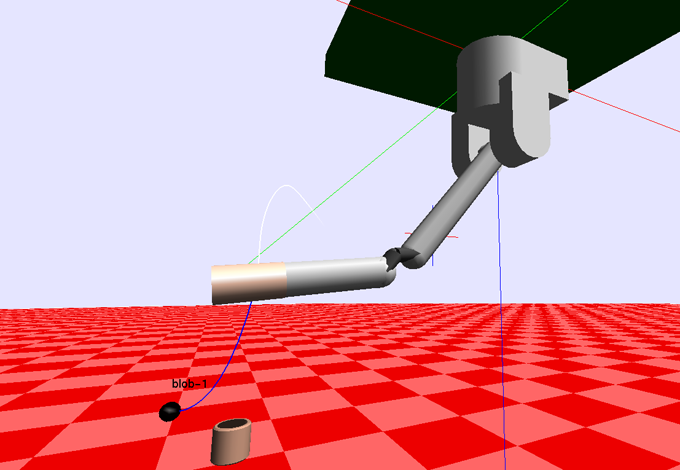
\includegraphics[width=0.8\textwidth]{Pics/Casting.png}
  \caption{A picture of the casting simulation.}
  \label{pic:casting}
\end{figure}
%
\textbf{Objective:} Guide a ball on a string into a cup on the ground. \\ \\
%
\textbf{Setup:} We use the WAM and fix an elastic string to its end-effector. At the end of the string we fixate a ball. On the ground we place 
a cup. \\ \\
%
\textbf{Description:} 
This task resembles the operation of a construction crane, as shown in Fig. \ref{pic:casting}. Instead of fixing a tool to the end-effector of the robot, an elastic string is 
attached directly to the robots end-effector. To the other end of the string a ball is attached. The objective of the robot is now to 
guide the ball into the cup placed anywhere on the ground inside the robots work space. The goal of the task is to put the ball in the cup as fast as possible which requires highly-dynamic movements. However, for fast movements of the robot the ball movement is very hard to predict. 
Thus, the problem is how to find a policy that moves the robots end-effector as fast as possible to the target 
position while introducing as little unpredictable forces to the ball as possible. 

This task can be adapted in terms of difficulty by adjusting the robots starting position, the string length and elasticity, as well as the 
diameter of the ball and the cup. 
\\ \\ 
%
\textbf{Code Dependencies:} The following task specific variables and function calls should be helpful to 
successfully complete the tetherball task. These are: \\
\begin{tabular}{ m{7cm} m{4cm}}
\begin{lstlisting}
Ball position
Cup position
Final reward
Simulate the physics
\end{lstlisting}
& \begin{lstlisting}
ball_state.x
cup_state.x
static double getRewardEpisode(void);
int sim_casting_state(int);
\end{lstlisting}
\end{tabular} \\


%%%%%%%%%%%%%%%%%%%%%%%%%%%%%%%%%%%%%%%%%%%%%%%%%%%%
%%%%%%%%%%%%%%%%%%%%%%%%%%%%%%%%%%%%%%%%%%%%%%%%%%%%
\newpage
\appendix

\section{Installation Guide}
%%%%%%%%%%%%%%%%%%%%%%%%%%%%%%%%%%%%%%%
SL supports all UNIX type operating systems (i.e. Linux, Mac OS) and is currently distributed internally. In addition to this guide, there exists a documentation by Stefan Schaal as well as some information on the on our website:

\begin{itemize}
  \item Documentation of the SL package \url{http://www-clmc.usc.edu/publications/S/schaal-TRSL.pdf}
%  \item Installation hints \url{http://ml.informatik.uni-freiburg.de/pub/learningrobots/simulator:installation}
  \item DoxyGen documentation of the SL package 
\end{itemize}




\subsection{Before Installing}
LINUX:
If you are using Linux, you will need to download some implementation of GLUT and X11:
\begin{lstlisting}
  sudo apt-get install xutils-dev
  sudo apt-get install libncurses5-dev 
  sudo apt-get install libreadline5-dev 
  sudo apt-get install freeglut3-dev
   
  sudo apt-get install tcsh
\end{lstlisting} 
%
MAC: For SL on Mac OS, you need
\begin{enumerate}
  \item install: readline either with MacPorts or Fink
  \item install: freeglut and freeglut-shlibs with fink a la
\end{enumerate}
\begin{lstlisting} 
sudo /sw/bin/fink install freeglut 
\end{lstlisting} 
%
If you are using a Mac, you will need to make some adjustment to the amount of memory your OS is willing to share. Go to the terminal and type

\begin{lstlisting} 
sudo vim /etc/sysctl.conf 
kern.sysv.shmni=128
kern.sysv.shmseg=32
\end{lstlisting}
%
Make sure you have the necessary tools installed for using and compiling SL code. SL uses iMake to ensure portability between different operating systems. iMake is part of the X11 distribution. If you are using a Mac, get the developer tools from the official Apple homepage or from the app store. You will need to register, but the tools are free of charge.

\subsection{Setting up SL}
To set up SL, download the archive from 
\begin{itemize}
  \item \url{http://www.intelligent-autonomous-systems.de/pmwiki/uploads/Teaching/RobotLearningProject/robolab.zip}
and extract the package into your home folder. The official document still refers to an installation using different users, this is obsolete in the current version.
\end{itemize}
%
For Mac AND Linux: You will need to copy and rename "dot\_cshrc" from robolab to the home folder as ".cshrc".
\begin{lstlisting}  
cp dot\_cshrc ~/.cshrc 
\end{lstlisting} 



\subsection{Compiling and running SL}
For Mac or Linux, it should be sufficient to first generate the config file
\begin{lstlisting} 
cd ~/robolab/shared/config
./SL-INSTALL 
\end{lstlisting} 
After confirming twice to set the install directories you have to start from the robolab root folder the './recompileSL.sh' script. Note that this only works in tcsh.
\begin{lstlisting} 
  tcsh
  cd ~/robolab
  ./recompileSL.sh
\end{lstlisting} 

\subsection{Run SL}
SL generates an individual executable for each robot. For starting the Barrett simulation, go to the `barrett' directory and run `xbarrett'
\begin{lstlisting} 
  cd ~/robolab/barrett
  xbarrett
\end{lstlisting} 
SL starts with 5 different console windows and 2 graphical output windows. You have one console window for each of the servos of SL. SL has 5 servos, the simulation, the openGL, the motor, the vision and the task servo.  The  user can enter commands
at runtime for each of this servo. You can find a list of all possible commands for a single servo by entering 'man' in one of the terminals. 
For us, only the simulation and the task servo will be of immediate interest. 
\subsubsection*{Simulation Servo}
Here you can set whether you want the simulation to run in real-time or with the fastest available computation speed. Entering {\em realTime} toggles this flag. In addition you can also change basic properties 
of the data logging mechanism of SL by calling {\em outMenu} (see Section \ref{se:SCD}).
\subsubsection*{Task Servo}
In the task servo you can choose which task you want to execute as well as apply basic commands to the robot or do some logging. The most important commands are
\begin{itemize}
  \item {\em st} : Set a user task which is subsequently executed. We refer to the next chapter for more details how to create an own user task. SL has 4 predefined tasks which are often
helpful for basic testing of robot models. The {\em Goto} task can be used to navigate the robot to a specified joint position, while the {\em Goto Cart} task navigates to a specified end-effector position in Cartesian coordinates. There is an additional 
task for loading and executing trajectories as well as performing sine-like movements with the joints. 
  \item {\em scds} : Start logging the joint angles and other variables which are subsequently stored in a Matlab file
  \item {\em where} : Prints the current joint positions of the robots
  \item {\em cwhere} : Prints the current Cartesian end-effector positions
  \item {\em ctp} : Change task parameters
\end{itemize}



\section{Adding a New Task to SL} 
Adding new tasks to SL is straightforward and thanks to iMake, it is also easily done for multiple platforms.
%%%%%%%%%%%%%%%%%%%%%%%%%%%%%%%%%%%%%%%
\subsection{Writing the Task-File}
If you want to add a new task to SL, you need to create a new C-file in the corresponding source code folder (in our case {\em barrett/src/}). The C-file has to contain 4 functions:
\begin{itemize}
 \item {\bf Initializing task variables: }
Whenever SL starts a new task it calls the initialization function of this task such that global variables can be properly initialized.
\begin{lstlisting}
static int init_mycooltask(void) 
{
    // initialize my variables here...        
}
\end{lstlisting}
 \item {\bf Controller function : } The controller function is executed for every simulation cycle. Here, the user can access the state of the robot and send commands to the robot. We refer to the following section for more details
on these functions. 
\begin{lstlisting}
static int run_mycooltask(void) 
{
    // Control the robot
}
\end{lstlisting}

\item {\bf Changing task parameters : } This function can be called by the user from the task servo terminal. Here you can read in new task parameters from the user.
\begin{lstlisting}
static int change_mycooltask(void) 
{
    // Read in some parameters...
}
\end{lstlisting}

 \item {\bf Adding the task to SL : } The add function has to be finally called by SL such that the task appears in the menu for choosing the tasks.
\begin{lstlisting}
void add_mycooltask( void )
{
    addTask("My Task", init_mycooltask, run_mycooltask, change_mycooltask);			
}    
\end{lstlisting}
\end{itemize}
You can use the file {\em templates/myCoolTask.c} as template file for creating new tasks.

\subsection{Adding the Task}
In SL, tasks are added through the {\em initUsersTasks} function. This function contains the calls to the user generated robot tasks.
\begin{itemize}
  \item  open the file {\em robolab/barrett/src/initUserTasks.c}
\end{itemize}
%
In the initUserTasks function body, add the lines:
\begin{lstlisting}
 extern void add_mycooltask(void);
 add_mycooltask();
\end{lstlisting}

\subsection{Adapting iMake}
Finally, the last thing you will have to do is to add the new source code file to the iMakefile:
\begin{itemize}
  \item Open {\em robolab/barrett/makefiles/imakefile.unix}
\end{itemize}
%
Under {\em SRCS\_XBARRETT} and {\em OBJS\_XBARRETT} respectively, add the lines
\begin{lstlisting}
  MeinBEISPIEL\_task.c \textbackslash
  MeinBEISPIEL\_task.o \textbackslash
\end{lstlisting}
%
That's it. Recompile, start SL and your new task should be there.




\section{SL data-types}
 We will first discuss basic SL data-types for the global variables and subsequently explain the most common SL function calls. 
Note that unlike standard C-arrays the indexing of SL-arrays (including the data-types Vector and Matrix) always starts at 1.
\begin{itemize}
 \item Vectors and matrices :
\begin{lstlisting}
typedef double*  Vector;
typedef double** Matrix;
\end{lstlisting}
Numerical computations with vectors and matrices are implemented with double pointers. SL provides all basic vector/matrix manipulation functions such as matrix product or the inverse of an matrix. For further  documentation
on matrix computations in SL please consult the doxygen documentation on the file {\em utility.h}.

\item Current Joint State :
The current robot state is stored in the global variable {\em joint\_state[]}. The array contains an {\em SL\_Jstate } structure for each DOF. 
\begin{lstlisting}
typedef struct { /*!< joint space state for each DOF */
  double   th;   /*!< theta */
  double   thd;  /*!< theta-dot */
  double   thdd; /*!< theta-dot-dot */
  double   ufb;  /*!< feedback portion of command */
  double   u;    /*!< torque command */
  double   load; /*!< sensed torque */
} SL_Jstate;
\end{lstlisting}



\item Desired Joint State :
We can set the desired joint position, velocities and acceleration with the global variable {\em joint\_des\_state[]} which is of the type struct {\em SL\_DJState}.
\begin{lstlisting}
typedef struct { /*!< desired values for controller */
  double   th;   /*!< theta */
  double   thd;  /*!< theta-dot */
  double   thdd; /*!< theta-dot-dot */
  double   uff;  /*!< feedforward torque command */
  double   uex;  /*!< externally imposed torque */
} SL_DJstate;
\end{lstlisting}
SL translates the desired joint state to the motor command by using an internal PID controller (see Section \ref{se:PID}). 

\item Current End-Effector Position :
The current end-effector state is stored in the global variable {\em cart\_state[]}.
\begin{lstlisting}
typedef struct { /*!< Cartesian state */
  double   x[N_CART+1];    /*!< Position [x,y,z] */
  double   xd[N_CART+1];   /*!< Velocity */
  double   xdd[N_CART+1];  /*!< Acceleration */
} SL_Cstate;
\end{lstlisting}
Acceleration is usually not precomputed as this is analytically too expensive. The velocities {\em xd} are calculated by the use of the Jacobian. 

\item Current End-Effector Orientation :
The current Euler angles and angular velocities are stored in the variable {\em cart\_orient[]}. 
\begin{lstlisting}
typedef struct { /* Cartesian orientation */
double a[N_CART+1]; /* Position [alpha,beta,gamma] */
double ad[N_CART+1]; /* Velocity */
double add[N_CART+1]; /* Acceleration */
} SL_Corient;
\end{lstlisting}
\end{itemize}
Before calling the user-provided {\em rum} function for a task, SL updates all these global variables such that they can be accessed by the user. Control of the robot is entirely implemented by
setting the global variable {\em joint\_des\_state[]}.


\section{Writing controllers} 
The controllers are implemented in the corresponding {\em run} functions of the task file. The basic communication with the simulated or real robot is implemented via shared memory. The state of the robot as well as the commands
to the robot are stored in the discussed global variables which can be accessed and modified by the user in the run function of the task.

\subsection{Internal PID Controller \label{se:PID}}
In SL the user can set the desired joint positions $\mathbf{q}_d$, velocities $\dot{\mathbf{q}}_d$ and accelerations $\ddot{\mathbf{q}}_d$. SL subsequently uses an internal PID controller to transform the desired joint configuration into a motor command.
\begin{equation}
 u = K_p (\mathbf{q}_d - \mathbf{q}) + K_d  (\dot{\mathbf{q}}_d - \dot{\mathbf{q}}) + K_i \int (\mathbf{q}_d - \mathbf{q}) dt + u_{\textrm{ff}}, \label{eq:PID}
 \end{equation}
where $K_p$, $K_d$ and $K_i$ are the PID controller gains and $u_{\textrm{ff}}$ is the feed-forward motor command\footnote{Which is usually set by the inverse dynamics calculation}. The used controller gains are stored in the file
{\em config/Gains.cf}.

\begin{lstlisting}
 /* format: keyword, gain_th, gain_thd, gain_int, max_control  */
R_SFE 200.     7.     .0   75
R_SAA 300.    15.     .0  125
R_HR  100.     5      .0   39
...
\end{lstlisting}
\subsection{Control Modes}
Besides the standard PID control mode, SL also easily allows for the use of more sophisticated control laws such as gravity compensation, feed-forward control and inverse dynamics. 
All modes can be implemented by a different use of the {\em SL\_InverseDynamics} function
\begin{lstlisting}
void SL_InverseDynamics(SL_Jstate cstate, SL_Djstate *dstate, 
                        SL_endeff *endeff,  SL_Cstate *base_state, SL_Corient *base_orient)
\end{lstlisting}
The function adds the feed-forward command {\em dstate[i].uff} to the desired state of the robot. The feed-forward command is subsequently added to the PID controller output (see Equation \ref{eq:PID}).
This function assumes that {\em dstate} already contains the proper desired position, velocity,
and acceleration for every DOF. The array of end-effector information is passed to
include possible external loads at the end-effector to the inverse dynamics computations. You can simply use the global variable {\em endeff} for this parameter. The variables {\em base\_state} and {\em base\_orient} provide the coordinates
and orientation of the robots base (needed for floating base robots). You can again simply use the global variables {\em \&base\_state} and {\em \&base\_orient} for this parameter. 

Depending on the arguments, the feed-forward signal calculated by {\em SL\_InverseDynamics} function implements 3 different control modes.

\subsubsection{Gravity Compensation Control}
Gravity compensation control counter-acts the forces introduced by gravity. In order to determine the gravity compensation part for the feed-forward command $u_{\textrm{ff}}$, we pass the current position with zero velocities as desired state, subsequently
we can use the returned $u_{\textrm{ff}}$ for our PID controller:

\begin{lstlisting}
// Compute inverse dynamics for dq=dqq=0 
for (i = 1; i <= N_DOFS; i++)
{
  joint_des_gravi[i].th = joint_state[i].th;
  joint_des_gravi[i].thd = 0.0;
  joint_des_gravi[i].thdd = 0.0;
}
SL_InverseDynamics(NULL, joint_des_gravi, endeff);

// Now fill in uff real desired state for PID control
for (i = 1; i <= N_DOFS; i++)
{
  joint_des_state[i].th = my_desired_position[i];
  joint_des_state[i].thd = 0.0;
  joint_des_state[i].thdd = 0.0;

  joint_des_state[i].uff = joint_des_gravi[i].uff;
}
\end{lstlisting}
Note that the current state argument for {\em SL\_InverseDynamics} is not specified in this case (NULL).

\subsubsection{Feedforward Control}
Feedforward control calculates the feed-forward command solely based on the desired target state, the current state is neglected (thus, no model-based feedback is used).
\begin{lstlisting}
// Compute inverse dynamics for dq=dqq=0 
for (i = 1; i <= N_DOFS; i++)
{
  joint_des_state[i].th = my_desired_position[i];
  joint_des_state[i].thd = my_desired_velocity[i];
  joint_des_state[i].thdd = my_desired_acceleration[i];
}
SL_InverseDynamics(NULL, joint_des_state, endeff);
\end{lstlisting}
Note that the current state argument is again not specified in this case (NULL).

\subsubsection{Inverse Dynamics Control}
Inverse dynamics control uses the known system model to determine the feed-forward command such that the real acceleration and the desired acceleration in {\em dstate} match. Thus, only the desired 
acceleration is used from the {\em dstate} variable is used. It is the most robust control method, however, it also strictly relies on an exact model of the system dynamics. 
In oder to implement inverse dynamics control we also have to pass the current state to {\em SL\_InverseDynamics}.
\begin{lstlisting}
// Compute inverse dynamics for dq=dqq=0 
for (i = 1; i <= N_DOFS; i++)
{
  joint_des_state[i].th = my_desired_position[i];
  joint_des_state[i].thd = my_desired_velocity[i];
  joint_des_state[i].thdd = my_desired_acceleration[i];
}
SL_InverseDynamics(joint_state, joint_des_state, endeff);
\end{lstlisting}
For standard PID control simply do not call the {\em SL\_InverseDynamics} function (i.e. set {\em uff} to $0$), just setting the variable {\em joint\_des\_state} is sufficient.


%%% SHARED MEMORY
%\subsection{Shared Memory Matlab Interface}
%In order to facilitate prototyping, a shared memory interface to Matlab is available in {\em sharedMemory.h}
%The shared memory code defines the following functions:
%\begin{lstlisting}
%int sharedMemReadDouble( int numValues, double * values);
%int sharedMemWriteResult(double reward);
%int sharedMemWriteData(double * data, int numValues);
%\end{lstlisting}
%
%Using this interface in SL could look like in the following:
%\begin{lstlisting}
%if( state == WAITFORDATA )
%{        
%	reward = 0.f;        
%	if( sharedMemReadDouble(3, gains) )
%	{
%		k               = gains[0];
%		d               = gains[1];
%		a               = gains[2];
%		gotoStartTime   = servo_time;
%		state           = CONTROL;
%	}        
%}    
%if(state == CONTROL)
%{   
%	//Control the robot        
%	reward += calcReward();
%	if(servo_time - startTime > 10.f)
%	{
%		sharedMemWriteResult(reward); 
%		state = WAITFORDATA;    
%	}
%}
%
%\end{lstlisting}
%
%To interface this with Matlab, a Matlab mex file is available, called {\em SharedMemMex.cpp}. The Matlab mex code 
%takes an array of values, passes it to the shared memory and waits for about six seconds for SL to write results back.
%An example Matlab code could look like:
%\begin{lstlisting}
%numTrials						= size(actions, 1);
%DONEMATLAB					= 99999;
%DONESL							= 99998;
%SHAREDMEMTIMEOUT		= 99997;
%
%for t = 1 : numTrials
%    flag = 1;
%    while (abs(flag - DONESL) > 1e-5) 
%        [flag reward(t)] = SharedMemMex( actions(t,:) );                   
%    end
%end
%
%\end{lstlisting}
%
%An example of using the shared memory interface can be found in the BallOnBeam task files. 

%%%%%%%%%%%%%%%%%%%%%%%%%%%
%% %% MATLAB INTERFACE
%% 
\section{Matlab Interface}
Since programming and evaluating new methods directly in C code can be slow and hard to debug, we provide an interface between Matlab and the SL simulation environment. 
The interface allows researchers to perform all learning operations in Matlab while still evaluating their policies in the realistic physics environment of SL, or even on a real robot. 
As real-time control of SL via Matlab would be too slow, we use a trajectory-based implementation. Each episode can be composed of several trajectory segments which 
are sequentially transmitted to SL. From Matlab, we can send a whole trajectory which is subsequently followed by a feedback controller
in SL. After the trajectory execution is finished, SL sends back all sensory information to Matlab for further processing. The interface can be used in two modes: SL can now either 
wait for Matlab to send a new trajectory (i.e., the SL simulation freezes) and subsequently continue the episode, or, the SL simulation continues with a default behavior (e.g., hold the position)
until Matlab sends a new command. Note that only the second mode is available at the real robot, but the first mode is beneficial for testing and prototyping, as the results are exactly reproducible
by retransmitting the same command sequence. 

The main component of the interface is a communication over shared memory which is protected by semaphores. Shared memory 
describes a part of the system memory that can be accessed by any program running on that system. Thus, if Matlab writes controller gains 
to the shared memory, SL can read out these controller gains and apply them to the robot. The advantage of shared memory 
compared to other possible solutions is that it does not introduce a time delay. 
%In order to use share memory between processes, it has to be allocated first. We provide methods that automatically reserve shared memory. The amount of shared 
%memory reserved depends on the number of degrees of freedom of the robot at hand as well as the predefined maximal number 
%of steps within one episode. To ensure robust and reproducible behavior of the interface, we employ semaphores to secure the communication. 

%Semaphores 
%are flags in the system that can be set by atomic operations.  These flags are used by the processes to determine whether they 
%currently have write and/ or read permissions on a certain part of the shared memory. Without these semaphores, two
%processes could try to write to the same memory location at the same time which could lead to undefined behavior. 
%Instead,  with semaphores, a process has to request write permission to the shared memory and can only get this permission, 
%if no other process is currently using it. If the process gets access permission, a flag gets set until the operation is finished. 

The main functionality of the shared memory system is implemented in {\em sharedmemory.cpp}. As Mac OS 
does not provide the same functionality as Linux based operating systems, some of the implementation is OS specific. 
The implementation provides functionality to allocate shared memory, attach it to a semaphore, lock and unlock the memory,
read and write to the shared memory and release the memory again.

\subsection{Shared Memory Matlab Interface}
Based on the described protected shared memory implementation, we provide the functionality to easily control SL via Matlab. 
On the Matlab-side of the interface, we provide `.mex' files that communicate with SL. Mex files are C/ C++ files that can 
be called directly from Matlab like normal Matlab functions. They take Matlab variables as arguments and also return Matlab 
variables. Each of the `.mex' files has a corresponding `.m' file which is wrapped around the `.mex' file for easier usability.  
To send data from Matlab to SL, the functions {\em SLSendTrajectory.m} and {\em SLSendController.m} can be used. SLSendTrajectory is used to transmit a whole trajectory segment, while
SLSendController can be used to transmit controller gains, for example, for the ball-on-a-beam task. 
For transmitting trajectory segments, we always have to specify the index trajectory segment within your episode we want to transmit. The index 
$0$ is reserved for sending the initialization commands for an episode to SL. Hence, the initialization segment usually only contains 
an initial position of the robot and also of the environment. If we do not send the indices of the trajectory segments in the correct order, SL
will think that there is a communication error and restart the episode. We also always have to  specify how many trajectory segments SL has to expect for one episode. After
executing the last trajectory segment, SL automatically automatically goes back to the initial state and waits for the initialization command ($\textrm{index} = 0$).
{\em SLSendTrajectory.m} takes the following arguments:
\begin{lstlisting}
[reward, state, flag] = SLSendTrajectory
	(trajectory, time, trajIdx, maxCommands, stateBuffer, timeOut)
\end{lstlisting}
%
\begin{tabular}{ m{3cm} m{7cm}}
\begin{lstlisting}
Inputs:
trajectory 
time
trajIdx
maxCommands
stateBuffer
timeOut

Outputs:
reward
state 
flag
\end{lstlisting}	 
&\begin{lstlisting}

The desired trajectory, that the robot should try to follow 
The number of seconds SL should wait before following the trajectory
The idx of the current trajectory inside the episode (typically 0 or 1)
The number of overall trajectories inside the episode
Memory for additional variables
A time-out Matlab should wait before assuming that SL crashed


The reward calculated by SL
The new state of the environment
A flag used to determine whether the episode was conducted without errors
\end{lstlisting}
\end{tabular}

In the interface, an episode describes one movement of the arm, such as a complete hitting movement. If the arm is 
to hit a ball twice the each hitting movement is one episode. The interface can be used to either send desired trajectories 
to SL, or to send controller gains. In the second case, the {\em stateBuffer} can be used to send the gains. 

If desired, the interface can also be used do read out all sensory values that have been measured during the trajectory execution. 
By calling {\em SLGetEpisode.m}, SL transmits the actual and desired joint angles, speeds, accelerations, the ball positions and any user defined variables 
are for each time step of the episode to Matlab. Such information can be useful for either 
defining a reward function in Matlab instead of SL or for debugging robot behavior. The Matlab and `.mex' files can be found 
in the directory {\em 'robolab/studentBarrett/Matlab'}. Additionally, files for testing the single tasks in Matlab are found in 
{\em 'robolab/Matlab/Test'}.

\subsection{Shared Memory SL Interface}

In SL, desired trajectories are read out from the shared memory and used to generate torques on the real or simulated robot. 
Since the structure of most tasks can be described in a similar pattern, we provide a state machine that has the desired 
functionality. The state machine is implemented in {\em SL\_episodic\_communication.c} and has four possible states: 
RESTARTEPISODE, GOTOSTART, WAITFORSTART and DOMOTION. While transitioning between these states, the state machine 
takes data from Matlab, performs the required motion and returns the new state as well as the reward calculated by SL to Matlab.
The state machine also ensures, that the robot will always start its movement from a predefined starting position, i.e., it will drive 
the robot to this starting position after each episode. 

Most tasks in SL provide a basic support for the Matlab interface. To do so, these tasks have to implement 
a specific set of functions which will be called by the state machine. As these functions are already implemented 
for the main functionality of the tasks, we only provide a brief description of these functions if a task needs to be extended. 



\begin{lstlisting}
void doMotionEpisodeStepExample(int commandIdx, double sendDataTime, int step)
\end{lstlisting}
Robot control during the execution of an trajectory segment is implemented here. 
Examples are, actually computing the desired 
torques for following the trajectory, 
calculating the reward or resetting values before starting a new episode.
\begin{itemize}
\item commandIdx: For reinitializing an episode, commandIdx is set to zero. Otherwise, it indicates the index of the trajectory
segment within the current episode. 
\item sendDataTime: how much time has passed since the last command was send FROM SL TO Matlab
\item step: How many steps the current trajectory segment was already executed
\end{itemize}

\begin{lstlisting}
int isStepOverExample(int commandIdx, double sendDataTime, int step)
\end{lstlisting}

The isStepOver function determines whether the execution of a trajectory segment has ended. 
Typically, a trajectory segment is terminated when we reached the end of the trajectory, but we could also want to wait for external events, e.g., observe the ball trajectory. 
\begin{itemize}
\item commandIdx: For reinitializing an episode, commandIdx is set to zero. In this case, isStepOver should return 1 if the start state have been reached by the robot. 
\item sendDataTime: how much time has passed since the last command was send FROM SL TO Matlab
\item step: How many steps the current trajectory segment was already executed
\end{itemize}

In order to access the data send to SL from Matlab, we can access the global variable {\em episodeTrajectory}. This variable always
contains the last command send from Matlab. The variable {\em episodeTrajectory} has the following elements

\begin{lstlisting}
typedef struct episode_trajectory
{
	int episodeID;
	int trajectorySize;// little steps
	int commandIdx;
	int maxCommands; // big steps
	double waitingTime;
	double trajectory[STEPLIMIT][N_DOFS + 1];
	double stateBuffer[NUMEPISODICSTATES];
} episode_trajectory;
\end{lstlisting}
The element {\em episodeID} is used for a fail-safe communication and not needed by the user. The other elements contain the {\em trajectory}, {\em waitingTime} is the time until
the trajectory is supposed to be started (typically not used), {\em stateBuffer} contains additional elements send by Matlab (see the {\em stateBuffer} argument for {\em SLSendTrajectory}).
The elements {\em trajectorySize} contains the number of steps of the trajectory transmitted by Matlab and {\em commandIdx} contains the index of the trajectory segment within the episode. 

In addition, the user can specify a function for storing data in shared memory. In the current implementation all common data such as 
joint positions, velocities, accelerations, torques, desired positions, velocities and accelerations are already stored, which is done by calling the 
function {\em writeStepToSharedMemoryGeneral}. Additional variables have to be added by a user-specified function
\begin{lstlisting}
void writeStepToSharedMemoryExample(int numStepInEpisode)
\end{lstlisting}
Used to store all relevant information in shared memory. The standard function is given by 
writeStepToSharedMemoryGeneral(numStepInEpisode), which should also be called by the user specified function.
The standard function already writes joint positions, velocities, accelerations, tourques, desired positions, velocities and accelerations.
Additional variables, such as a ball position, have to be written by the user defined function. 

To store data to shared memory, we can again use a global variable {\em episodeStep} which is of the type 

\begin{lstlisting}
typedef struct episode_steps
{
	int episodeID;
	int numTransmittedSteps;
	
	double joints[STEPLIMITEPISODE][N_DOFS];
	double jointsVel[STEPLIMITEPISODE][N_DOFS];
	double jointsAcc[STEPLIMITEPISODE][N_DOFS];

	double jointsDes[STEPLIMITEPISODE][N_DOFS];
	double jointsVelDes[STEPLIMITEPISODE][N_DOFS];
	double jointsAccDes[STEPLIMITEPISODE][N_DOFS];

	
	double torque[STEPLIMITEPISODE][N_DOFS];

	double cart[STEPLIMITEPISODE][3];
	double state[STEPLIMITEPISODE][MAXEPISODESTATES];
	
	int commandIdx[STEPLIMITEPISODE];
	
} episode_steps;
\end{lstlisting}
Additional variables can be stored in the element {\em episodeStep.state}. All other variables are 
already stored by the {\em writeStepToSharedMemoryGeneral} function, however, the  {\em writeStepToSharedMemoryGeneral} function
needs to be called in the user-specified {\em writeStepToSharedMemory} function.

After implementing these functions, they still have to be passed to the shared memory. This is simply done by calling
\begin{lstlisting}
 episodicSharedMemoryWait(&doMotionEpisodeStepExample, &isStepOverExample, 
&writeStepToSharedMemoryExample, &simPhysics, 0, 0)
\end{lstlisting}

in the {\em run} function of the task. The shared memory system can additionally be used to attach 
other processes, such as a vision system to SL and Matlab in a straightforward 
fashion.



\section{Inverse Kinematics}
In inverse kinematics we want to calculate the desired joint velocities given the desired task space velocities (velocities of the end-effector). 
SL offers an easy access to all quantities for calculating an inverse kinematics controller. The Jacobian for the current joint position is always stored in
{\em J[index\_task\_space][index\_joint\_space]} which is of the type {\em Matrix}. This can be used to implement any inverse kinematic control law such as the Jacobian Transpose 
or the Jacobian Pseudo-Inverse approach. In order to do so, the utility functions for matrices might be useful. 


\subsection{Determining the joint position for a desired end-effector position} 
Often it is also desirable to determine the joint position which implements a desired end-effector position and which is at the same time closest to some
rest-posture (since the mapping from end-effector position to joint position is not unique). This is done by the function 
\begin{lstlisting}
int inverseKinematics(SL_DJstate *state, SL_endeff *eff, SL_OJstate *rest,
		  Vector cart, iVector status, double dt)
\end{lstlisting}
The function calculates the inverse kinematics by using a damped pseudo-inverse approach. Starting from the joint positions given by {\em state}, it determines the Jacobian, calculates the pseudo-inverse in order to get the joint velocities
and already integrates the velocities with time step {\em dt}. The parameter {\em rest} defines the resting position of the robot, this is used as additional optimization in the null-space of the Jacobian to additionally minimize the distance
to this position. The {\em SL\_OJstate} structure also already contains a weighting of each joint dimension. The vector {\em cart} defines the error of the Cartesian state of the end-effector (position and orientation), with {\em status}
we can disable certain Cartesian coordinates (e.g. the orientation). 

If we want to determine the joint position  given the Cartesian coordinates of the end-effector, we can iteratively call this function. In addition the auxiliary functions {\em linkInformationDes, linkQuat, jacobian} are useful to determine the Cartesian coordinates for a given
joint position, the quaternion and the jacobian for a given joint state. Please consult the doxygen documentation for more details on these functions.

\section{Data analysis \label{se:SCD}}
SL already includes many tools for data analysis which are based on Matlab. By calling {\em scd} (or typing it in the task servo)  SL starts the data collection. SL automatically stores the data in a Matlab format such that it 
can be easily analyzed. SL stores all relevant variables such as joint and end-effector position, velocities and accelerations. It is also possible to add user defined variables to the data collection. This can be done by the functions
\begin{lstlisting}
void addVarToCollect(char *data_ptr,char *name,char *units, 
                     int type, int flag);
\end{lstlisting}
which is usually called in the {\em add\_task} function. The parameter {\em data\_ptr} has to point to the desired variable (only global variables are allowed), the parameter {\em name} defines the name of this variable, and {\em units} the type of unit (both are strings). {\em type} specifies
the type of the variable which is one of DOUBLE, FLOAT, INT, SHORT and LONG. At the end of the {\em add\_task} function the function {\em updateDataCollectScript()} has to be called to initialize the data collection script. 

In addition to calling the {\em addVarToCollect} function all variable names have to be specified in the script file {\em prefs/sim\_default.scipt}. The script file, the sampling time and the sampling frequency can additionally be defined by
calling {\em outMenu} in the motor servo shell. 

The data files are usually stored in the root directory of the robot. They can be easily loaded and analysed in Matlab by calling {\em clmcplot} which is located in {\em robolab/matlab/clmcplot}.



\bibliographystyle{ieeetr}
\bibliography{Bibliography}


\end{document}  